\chapter{Results}\label{cha:Research}
%

% Ska följa som ett naturligt komplement till huvuddelen

In this chapter, the results are presented, so that in the next chapter, these results are analysed. \todo{Flytta Insights som besvarar en Research Question till Discussion, och hänvisa till iteration. I Resultat vill vi bara ha Resultat, ej svar på forskningsfrågor, så spara svar på forskningsfrågor tills Diskussion.}

%\section{Example}\label{sec:research:history}
%
Liksom \citep{Duck:2005} har vi kommit fram till att glass smakar bäst på sommaren \citep{Khalil02NonlinearSystemsBook}.

\marginpar{Kommer att tänka på en liten anekdot\ldots}

\Warning[TODO]{Ta bort den löjliga anekdoten!}

\begin{figure}[tbp]
  \centering
  \subfloat[Alldeles för tidigt.][\label{fig:times:very-early}Det här är väl tidigt — din glass hinner smälta innan ditt sällskap dyker upp.]{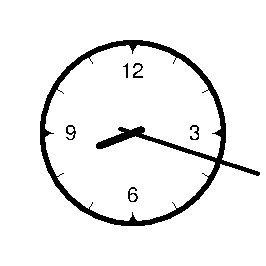
\includegraphics[page=1]{clocks}}
  \qquad
  \subfloat[Med marginal.][\label{fig:times:early}Kiosken stänger snart, men inte nu — perfekt!]{\includegraphics[page=2]{clocks}}
  \\
  \subfloat[I grevens tid.][\label{fig:times:on-time}Precis i tid — du får in ett finger i luckan just när kiosken ska stänga.  Han som jobbar blir sur, och det blir smolk i bägaren.]{\includegraphics[page=3]{clocks}}
  \qquad
  \subfloat[Försent.][\label{fig:times:late}Du är sen — kiosken är stängd.]{\includegraphics[page=4]{clocks}}
  \caption{\label{fig:times}%
    Illustration av \emph{subfloats}.  Den så kallade \emph{bounding box}en visas i \protect\subref{fig:times:late}.  Lägg märke till att bounding boxen har satts så att alla bilder har samma storlek, med enhetlig placering av själva innehållet i förhållande till bounding boxen.  Antag att du ska träffa en kompis för att äta glass just när kiosken stänger för dagen vid 08:30.  När dyker du upp?}
\end{figure}

\section{Developed Application}

  In figure~\ref{fig:iteration-map} the end results of the app from iteration 1, 2, 3 and 4 are shown. The final app works on web or as an app, online or offline, on all of YoungDrive's Android and iOS devices. The app is fast to use, the back button on the phone can be used to go to the previous view, and the font size and images are consistent for each screen (which was not the case iteration 1-3, see figure). The goal was to provide a great learning experience, with a strong YoungDrive feel (embracing the values of fun, plus using the YoungDrive logo and colors)

  \begin{figure}[h]
    \centering
    \includegraphics[width=1.0\textwidth]{IterationMapLowRes.png}
    \caption{The app flow described as a timeline (A-I), per iteration (1-4). E.g. in iteration 4, login (B4) appears after choosing quiz to take (A4).}
    \label{fig:iteration-map}
  \end{figure}

  %\subsection{Iteration \#1}

  There was no developed application at this point.

  Instead, two workshops were held, which together would inform the future development of an application.

  There were the findings from those two workshops:

  \subsubsection{Workshop \#1: Customer Journey Map: A day as a coach}

  \subsubsection{Workshop \#2: Quizical and Duolingo}



  The quiz flow iteration 1-2 was a standard multiple-choice quiz game, designed for assessment, but not for learning. In a scoreboard, they could see which questions they were awarded points for and not, with a total score. In the end of iteration 2, whey were encouraged to go back to the start screen, to redo the same quiz again, or select a new one.

  %\subsection{Iteration \#2}

  \subsubsection{Result}
  Quiz-flödet 1.0: standard multiple-choice, designat för assessment, men ej för learning
  Besvara multiple-choice-frågor
  Få resultat-tavla med Question 1: 0, Question 2: 1, samt "Total score: X/X"
  Gå tillbaka till startskärm

  \subsection{Iteration 3}

  \subsubsection{Result}

  Quiz flow 2.0 was designed for learning and self-reflection

  \begin{itemize}
  \item vid varje fråga besvarar du det alternativ du tror är rätt samt "Are you sure?" Yes/No
  \item vid färdigt quiz, få en resultattavla med personliserad feedback
  \item läsa igenom dina felaktiga svar och hur säker du varit på dem
  \item observerat de korrekta svaren
  \item klicka "Improve" för att bara få dina felaktiga svar igen
  upprepa tills inga felaktiga svar var kvar (det står "quiz try: 3", om det är försök 3)
  \item vid 100%, låsa upp "I can get 100%" (som är hela quizet igen)
  \item innan dess, uppmuntrades du läsa igenom coach/deltagar-manualen
  \item om du då fick något fel, fick du gå tillbaka till träning igen
  \item om alla rätt på, blev du Certified coach. Om du klarade det på första försöket, fick du även en guldstjärna (andra försöket = silver, tredje försöket = brons)
  \item sedan kunde du ta ett annat quiz
  \end{itemize}

  Kommentar, fördelar med feedback-läge:
  Genom att på varje fråga besvara "Are you sure?": Yes/No, så stärker vi inte bara coachens meta-kognitiva förmåga, utan vi kan vi även ge personliserad feedback i resultattavlan, istället för att bara visa Question 1: 1 point. Question 2: 0 points, som i Iteration 2.

  Detta gör att coachen kan reflektera över sitt lärande på t.ex. följande sätt:
  - få en självförtroende-boost (via feedback "You were correct, and you were sure")
  - gå från gissning till självsäkerhet (via feedback "You guessed, but you were correct")
  - ändra uppfattning snabbare (via feedback "You were incorrect, but you were sure")
  - uppmuntra coachen att läsa i manualen (via feedback "You were incorrect, and you were not sure")

  Fördelar med tränings-läge, och certifikations-läge:
  From Josefina: "Jag gillar idén att när coachen har kunnat svara rätt på alla frågor, kunna befästa kunskapen med hjälp av certifikations-läget, då coachen ska kunna få 100\% rätt på 1 försök."

  \subsection{Iteration \#4}

  %Result

  \todo{Show images of final app - on mobile, tablet and desktop?}


\section{Iteration 1}

Here the results from the qualitative and quantative data for iteration 1 are shown, together with conclusions.

\subsection{Qualitative data}

\subsubsection{Entrepreneurship education considerations}
Throught early interviews with YoungDrive staff, it is clear that YoungDrive's entrepreneurship education methodology goes hand in hand with the presented theory. It's mottos are: "Dream big, start small", "Learning by doing" and "We have fun!" \citep{youngdrive}.

Both in regards to designing for the users and for the above reason, the app should be a complement to YoundDrive's existing training material and the structure of the program.

A challenging part of the work is that YoungDrive consists of both the practical skills of the entrepreneur, theoretical material of running a business, and an entrepreneurial mindset. Therefore, both how to assess knowledge, and build habits, needs to be examined.

\subsubsection{Understanding the coach situation}

A CBT can be responsible for from 7 up to 12 different youth groups in different programs, and such a high number places huge demands on the CBT.

Even if there are only 7 groups, being behind on schedule or not being confident, can be very demanding.

\textbf{Stayover at Patrick:} På morgonen visade Patrick mig hur han jobbar med deras tomt, var det odlas ris, och andra råvaror, deras djur, deras story från Syd-Sudan, till Kampala, till hyddan här i Tororo, och hans värderingar.

Efter en ungdomssession nästföljande dag besökte vi och hälsade kort på en av de 2 CBT:s vi har session med idag. Sedan hade jag och Patrick den obligatoriska review av ungdoms-sessionen, och jag bjöd honom på middag. Kl. 19 ringde hans fru (som har börjat få tecken av malaria) och skyndade hem.

Nästa ungdomssession fick jag besöka en annan CBT. Vi var tidiga. Sedan började jag prata med henne, och fick bra tillfälle att intervjua henne och även förklara för henne vad jag gjorde där. Det blev underligt att förklara för henne: Patrick påminde, när jag tabbat mig, att “Marcus, du måste förklara för X vad en app är”. Så hon fick låna min mobil, och jag förklarade att app var kort för applikation, och att för varje applikation har ett eget syfte, t.ex. ta foton. Jag bad henne klicka, svårt, råkade klicka åt henne, men sedan lät jag henne göra. Efter hon sett att det hon såg i skärmen var det hon såg på riktigt, blev hon jätteglad och började fundera vad hon skulle fota. Hon reste sig och gick runt hörnet, och jag följde efter. Hon fotade, efter att noggrannt tänkt igenom, att hon fotade buskarna med frukt. Sedan sade jag hon kunde fortsätta fota, och då tog hon ett litet runt hus utanför.


\subsubsection{Different kind of coaches}

The interviews with CBTs, PLs and stakeholders led to the realization that different coaches handles this differently well.

Depending on the situation, e.g. you are not confident, or you are falling behind with the schedule, you can be in one of these need groups.

\begin{itemize}
  \item The ideal coach
  \item The realistic coach
  \item The challenged coach
\end{itemize}

It was discovered, that coach confidence comes largely from being able to have good youth sessions.

\subsubsection{A good youth session}

For having a good youth session, these are the most important attributes:

\begin{itemize}
  \item Correct information
  \item Correct structure
  \item Time management
  \item Fun atmosphere
\end{itemize}

The fact that the coach knows they have these qualities, leads to self confidence from the coach. This in turn, leads to better meetings with the youth.

\subsubsection{The room for a digital solution}

It is definitely a problem that so extremely few have smartphones.

This needs to be designed for. Either, I build only for the use case of having an app tailored for the coach training, where the donated devices can be used.

Alternatively, I design only for the users that does have a smartphone, and count that more will get smartphones in the future.

Thirdly, I can use a SMS tool, not building an app but an SMS-based service, which also could be an app. Such tools exists, and are compatible with multiple-choice questions, like VOTO Mobile.

\subsection{Iteration \#1}

    %What the data said

    \subsubsection{Results from the coaches}

    \subsubsection{Observable trends from the coaches}

\subsection{Iteration \#1}

\subsubsection{Motivation of app}
The scope of the app is to examine and strengthen the entrepreneurship the student already has. One important goal is to give good feedback.

The users are already motivated. Thus, I can follow Sierra's advise designing for the compelling context.

My compelling context is that I want to help you become an even better coach.

The better user point of view: don’t just make a better coach training app - make a better user of coach training material.

For me, this means:

"Given a teaching situation among the youth group, a great coach can teach an entrepreneurship topic more consistent with what the coach material said."

"Given a question in the app, a great coach will get the right answer more often, and increasingly leverage the correct answer to their coach situation."

\subsubsection{Entrepreneurship education considerations}
The YoungDrive's entrepreneurship education methodology goes hand in hand with the presented theory. It's mottos are: "Dream big, start small", "Learning by doing" and "We have fun!" \cite{youngdrive}.

Both in regards to designing for the users and for the above reason, the app should be a complement to YoundDrive's existing training material and the structure of the program.

A challenging part of the work is that YoungDrive consists of both the practical skills of the entrepreneur, theoretical material of running a business, and an entrepreneurial mindset. Therefore, both how to assess knowledge, and build habits, needs to be examined.


\section{Iteration 2}

Here the results from the qualitative and quantative data for iteration 2 are shown, together with conclusions.

\subsection{Qualitative data}

\subsubsection{Design workshop \#1 in Zambia}

The result was fantastic, in the sense that it gave me an unbiased look at what the coaches expected from the app, what functionality wasn't important, and into their technical preferences.

The designs and insights gained were used throughout the week to further improve the app I had actually started creating, and gave great insights to who the coaches were and their thinking. \todo{Add image here}

\subsubsection{The desire perspective}

Insight: "The app could be used on my spare time". This is particularly true, about the bonus quizzes that were produced during the week.

Insight: \textit{Coach:} "I'll buy one" (a smartphone), \textit{Response from other coaches: } "Whoa!"

\subsubsection{The utility perspective}

Ideation: "The app should have notes, not only quesitions"

\subsubsection{The usability perspective}

Low resolution screens, made the text be barely visible. This showed, that the app needed to be tested on a lot of different devices. This is particularly true, as on day 1, the coaches did not know how to zoom, which could cause accident refreshs, frustration or confusion.

The app needs to work offline! To be online on the phone is too expensive for the coaches, and too unrealiable to give a satisfactory experience. Also, during testing, relying on internet can cause a lot of problems, especially if the teacher is alone.

\subsubsection{The learning perspective}

    The coaches had surprisingly high results, and at day 3 they wished harder questions when asked.

    We responded by having harder questions, e.g. by introducing similar answers, and testing 4 alternatives instead of 3. This was appreciated.

    The following analysis could be done:

    \subsubsection{Doing a pre-quiz: good for learning}
    When asked about what they thought about doing "Graduation" as a pre-quiz (before the session), 10/10 said they liked doing the quiz before, and that it benefited their learning during the session.

    When asked why it helped, these were the results:

    \begin{itemize}
    \item "During session, it is easier to follow" - 10 (100\%)
    \item "Giving the paper manuals before, scanning headings and pictures etc, would not help" - 10 (100\%)
    \end{itemize}

    It was also tested to work in group or individually. The ones who answered, said that you learned more individually (3/3), and more fun doing it together (3/3). Doing it together, was enjoyable as it was "Very easy because of using different minds" and "We can collaborate to do better".

    \subsubsection{Doing a post-quiz: Spaced versus massed learning}
    In "Goal setting", quotes were "I thought it was fun and challenging to do the quiz immediately afterwards", with another coach commenting "The mind was still fresh".

    When asked on timing preference, 10/10 said it would be more fun to do the quiz immediately afterwards, not at the end of the day. The motivation, seemed to be that it was easier.

    9/10, said they wanted to do the quiz afterwards. The outlier, said it would be better for learning doing it later.

    After this comment, this was the distribution:

    \begin{itemize}
    \item 3/10 wants to do the quiz both before and after a session
    \item 1/10 wants to do the quiz before and at the end of the day
    \item 7/10 wants to do the quiz only immediately afterwards
    \item 10/10 wants to do the quiz immediately afterwards, and then again at the end of the day
    \item 7/10 wants to do the quiz immediately afterwards, and then a joined quiz with other topics at the end of the day
    \end{itemize}

\subsubsection{The teacher perspective}

  \textbf{Low scores}
  The 9/19 shows the relevancy of the quiz, as Josefina did not think she would have discovered that the coach was lagging behind otherwise.

  In the data, it was observable that the coach had done well together with others, but 3/7 when done individually.

  Josefina said about the 9/19: "This is where a control group would be beneficial". "He is often passive during open questions, but active during the team exercises."

  The question we needed to ask ourselves, was: "Does this imply he is a good or bad coach?".

  \textbf{What would hinder Josefina from using the app}

  Josefina says: "Not doing data collection digitally works whenever they are 10 - but not with bigger numbers than that."

  According to the final interview with Josefina, she does not wish the app to replace her. She enjoys teaching, thinks she has an important role, and suggests the app to be designed to support her and the coaches, not replace her.

  \textbf{Acceptance criteria}

  If you have a high score, you are ready. If not, you need to redo the quiz.

  If you are 8/10 or lower, you are in the red zone. If lower than 10/10, they are not ready, the motivation being that what they don't know, they will teach in an improper way: affecting hundreds of youth. This is why Josefina thinks they should need all of the answers correct.

  \textbf{Testing Correct Structure, Time Management and Fun Atmosphere}
  Josefina informs that Correct Structure, Time Management and Fun Atmosphere would be the most valuable to test after a youth session. She also notes, that \textit{some} aseessment could be made via the app before a session. Because of the reason that this thesis does not focus on after-session-evaluation, Correct Information is primary to improving on the other factors, which are secondary.

\subsubsection{The developer perspective}

  \begin{itemize}
    \item Bugs was a big hindrance to functionality, and a lot (both high-dose, and high-scale) of testing is very important
    \item Simpler design than I thought (KISS) was sufficient
  \end{itemize}

\subsubsection{Bonus results: Testing the app on Kampala university student}
The app was tested on a university student from Makarere University.

The university student from Makarere University scored 100\% correct, in spite of not having any entrepreneurship training. This showed that guessing was possible, or that the quizzes were too easy.

\subsection{Quantative data}

    %What the data said

    \subsubsection{Results from the coaches}

    \subsubsection{Day 2}
    Most coaches prefer tablet: 5 prefer tablet, 2 smartphone, and 2 computer.

    \subsubsection{Day 3}
    iOS no longer allows uncertified app install from computer: you need to have paid a license even for unreleased apps, being a "Trusted developer". This stops the app from being able to be installed on all the iOS devices, so that only the web version can be used.

    Thus, only the web app was tested from Wednesday and onwards.

    This was a problems, as the app regurly crashed at refresh because of low internet capacity.

    Sometimes, it was neeed to go to the other office where there was wifi, to refresh the webpage, and go back to the location. This of course would not work for Josefina.

    \subsubsection{Day 4}
    Tested using the quiz before the session.  Using the quiz before the session increases learning, slightly decreases fun of the session, according to coaches. It is "Fun and encouraging".

    \subsubsection{Day 5}
    On day 5, the schedule was:

    \begin{itemize}
      \item "Goal setting" part 2
      \item App test: "Goal setting" after-quiz and "Graduation" pre-quiz.
      \item "Graduation"
    \end{itemize}

    In "Goal setting", one coach were an outlier to the other high results, scoring 9/19 answers correct.

    \subsubsection{Results from workshop \#2}

    During this workshop, the focus was to examine what builds confidence among the coaches. The following clusters could be determined: "I believe in myself" (3 coaches), "I believe in God" (2 coaches), "I am well prepared" (4 coaches) and "I am certified" (1 coach). \todo{Lägg till bild här}

    \subsubsection{Bonus results: Testing the app on refugee innovations}
    Back in Uganda, a test was done with refugee innovators, at the Humanitarian Innovation Jam.

    The test with the refugee innovatiors were surprisingly intriguing and successful.

    It was found that refugee innovators says they would have a great need for such an app.

\subsection{Iteration \#2}

\subsubsection{Insights}

The app works for assessment!

  Using the quiz before the session increases learning, slightly decreases fun of the session, according to coaches

  Fun and encouraging

  \begin{itemize}
    \item The app works for assessment!
    \item Good for learning for the coaches
    \item A good indicator for Josefina
    \item A great way to scale the YoungDrive training in the future, both for online coach-training and the physical training
  \end{itemize}

After the meeting with the partner and expert group, the following was concluded from iteration \#2:

\begin{itemize}
\item The app is only working on assessment now, not for learning
\item The need for a field app still feels relevant (especially for sessions long since the coach training)
\item The potential for YoungDrive having online coach training is huge
\end{itemize}

Determine:
\begin{itemize}
  \item Focus for the next iteration: design quiz app for learning, focus on field app (CI, CS, TM, FA), and design having an app that works stand-alone from the YD coach training in mind.
\end{itemize}

Discussing the importance of self-reflection after a youth session with Josefina, led to asking more of such questions in coach quizzes.

Josefina: “I have a problem: there is no way I can control them how they have prepared themselves for a youth session."

An app could be used, either before you start planning (to guide what you need to study the most on), or after you think you are ready (so you can assess and improve).

\subsubsection{Bonus results: Testing the app outside the YoungDrive context}
Back in Uganda, a test was done with refugee innovators, at the Humanitarian Innovation Jam.

Also, the app was tested on a university student from Makarere University

The test with the refugee innovatiors were surprisingly intriguing and successful.

It was found that refugee innovators says they would have a great need for such an app.

The university student from Makarere University scored 100\% correct, in spite of not having any entrepreneurship training. This showed that guessing was possible, or that the quizzes were too easy.

\subsubsection{Findings}

Test with university student scored 100\% correct, means that common sense can go a long way, and that the results can't be 100\% trustworthy, and that multiple-choice questions has serious issues - this, we already knew during and before the coach training - but it needs to be taken care of

The app would be great and could actually work outside the physical coach training - with revision, be stand-alone, even being able to distribute online.

Now there are observable evidence for what the interactions from Iteration 1 showed:

\begin{itemize}
\item The purpose of the coach training should be to prepare the coach in having great youth sessions
\item Therefore, this is what the quizzess should assess
\item What it really means being a good YoungDrive coach, is having good youth sessions
\item Josefina would have liked to be able to stop coaches from having taught, if they do not have 90-100 \% correct information on the subject
\item Today, Josefina can not assess this. This means that some coaches, are teaching incorrect information to hundreds of youth.
\item Here, the quiz has a very good need to fill.
\end{itemize}

With all of these findings in summary, it can be concluded that an app for coach training, and an app to use before a youth session, could be the same app, since the purpose of preparing the coach to be great with its youth session is the same.

From the interviews, it was learned that while it \textit{may} be technically possible, the teacher desires the app support her, not replace her.


\section{Iteration 3}

Here the results from the qualitative and quantative data for iteration 1 are shown, together with conclusions.

\subsection{Qualitative data}

  %What the observations said

  \subsubsection{Observations from Kampala test}
  The entrepreneurship student in Kampala, informed the following changes:

  Instead of "Become certified", he would be more motivated by unlocking the opportunity to apply the skills.

  "Improve" should be renamed "Try again", because it is more intuitive.

  His overall opinion on the app was:

  "Can you give me the link, because I'd love to do more of this. I think it's amazing."

  \subsubsection{Verified relevancy of seperating Training and Certification}
  When asked for an opinion, Josefina answered: "I like the idea that when the coaches have answered all of the questions correctly, they can consilidate the knowledge by the certification test, when the coach should get 100\% correct on their first try."

  \subsubsection{Field visits}

  The first thought was to use Gold/Silver/Bronze in the Training mode, and "Are you sure?" in the Certification mode. User tests showed that the other way around was better.

  \subsubsection{Big app test}
  \textbf{Learning: } The app test simulated the app being used to assess preparedness for a youth session. They clearly showed evidence between the difference between designing for Assessment and Learning:

  Given a coach having prepared for their youth session on week 9, and then only scoring 5/10, what should happen? In a similar way, what should happen if 9/10 correct answers?

  For the coach training, the assessment was okay, since Josefina could pick up and give feedback.

  Before a youth session, leaving the coach there is not viable. If the coach has 9/10, that coach should not only be let be, and especially if the score has been 5/10.

  Feedback was that one user did not want to press "Improve", until having read the manual. The motivation was: "Not because that is what the info says, but because I can learn more from the manual, about more than what the questions says."

  This is indeed the preferred behaviour from Josefina, and the app should continue to encourage only using the app training or certification mode after having prepared via the manual. This way, the app is still assessment, but it is "learning by thinking", with feedback.

\subsection{Iteration \#3}

    %What the data said

    \subsubsection{Observable trends from the coaches}

     \textbf{Usability: } The most notable thing from the app test, was that the app was not user friendly at all for 1st-time smartphone users. There were a lot of bugs, e.g. resizing of the font size for each new question. This forced some coaches to try to zoom on the devices, even if they did not know how. This could in turn cause refresh of the web page, and sometimes there was no Internet available. Thus, the data can not be fully reliable.

  This was the first time true frustration was shown. Out of 23 respondents, 7 rated the app easy, 11 medium, and 6 hard. This was not viable.

    \textbf{Related to mobile experience}
    Before the quiz started, the coaches were asked to raise their hand if they felt proficient with using a smart phone. 8 out of 23 said yes.

    After the quiz, 16 said they were proficient (25\% increase), while 5 said low proficiency, and 2 said no (we don't yet feel proficient, still fear).

    \textbf{Field tests}
    During field tests, 3 CBTs were visited, to further observe usage of the app after having prepared a youth session.

    Some things were notable from the interactions with John:
    \begin{itemize}
    \item "Are you sure?" is understood intuitively (you can't progress without answering), but some coaches deliberately answer "Yes" even if they are not sure.
    \item Idea to highlight different words of similar answers, to increase speed
    \item In summary, if wrong, show the other alternatives either way, not only the wrong answer
    \end{itemize}

    It was also here, that it was first observed that this is a light version of both deliberate practice and perceptual exposure. It is just that the app as of now is quite inefficient, especially in terms of speed.

    \todo{Add idea for future work: Show how a persons correctness level has increased over time}

    From the interactions with Juliet, this was discovered:

    \begin{itemize}
    \item Idea for future work: "Go to participant manual" within the app
    \item If correct and unsure, she says "I still feel good". "Include it in wrong, because maybe I was still guessing". (This later informed the Certification quiz-insight)
    \item Change button to "Become certified", to increase likelihood to press the button. As of now, it was not obvious.
    \end{itemize}

    When she did get certified, she said "I feel good". When asked why, she said: "They have appreciated what I have done".

    \textbf{"Are you ready?" app test}
    The next day, the three CBTs gathered at the Plan International office to do an app test on the hardest quiz.

    \todo{Add results}

\subsection{Iteration \#3}

  The app works for assessment!

  \begin{itemize}
    \item The app works for assessment!
    \item Good for learning for the coaches
    \item A good indicator for Josefina
    \item A great way to scale the YoungDrive training in the future, both for online coach-training and the physical training
  \end{itemize}


\section{Iteration 4}

Here the results from the qualitative and quantative data for iteration 4 are shown, together with conclusions.

\subsection{Iteration \#4}

Everyone now thought the app was good and easy to use.

With the Plan Tororo staff, it was shown how important the certification mode was: even though one group had 100\% on their first try, and a person had 1 wrong answer, the person with 1 wrong answer got 100\% on the certification, while the 100\% group had 1 wrong answer.

It is therefore determined, that when all of the answers can be answered correctly, after having gotten all answers correct once, that the knowledge is reliable - this is deliberate practice.

\subsection{Quantative data}

    %What the data said

    \subsubsection{Results from the coaches}

    \todo{Add table from Google Sheets}

    % Christine och Patrick berättade senare att i regel presterar Young Mentor lite bättre än CBT, enligt deras rakningar. (från iteratoin 1 - stämde detta?)

    Relevans av att testa financial literacy: "Precis som med förra gruppen, verkar ekonomin vara det svåraste att förstå (dolda utgifter, hur gå med vinst), som youth." (från iteration 1)

    \subsubsection{Data observations}

% Important to be objective
% En diskussion om hur resultaten kan användas i praktiken är också i de flesta fall belysande och relevant i rapporter

% https://liu.se/ias/kontakta-oss?l=en

In this section, the conclusions from the different group characteristics are presented.

Early observations from the pre-test data was that a surprising number of cells were left blank. One user had not done the pre-test, where some had left questions unanswered (most commonly "Do you own a company?" (should have used the word "business"), plus "Hours of preperation" and "Occations for a youth session" (there is a tendency this might be because they were not proud of their answers, because of correlations with low quiz results).

Missing cells was not as obvious with the app results, were users could not progress in a quiz without answering both the question and the confidence. However, none of the passed quiz 9 certification answers had been submitted. Thus, it was needed to add these from the manual recordings, which had been used as a backup in case anything like this would happen.


There were a number of quick insights that could be drawn before the parallell coordinates visualization: there was a surprisingly low number of answers where the user answered the question without confidence. Also, more users had started a quiz without finishing it than anticipated. Finally, a lot of users had done quizes that were not Topic quiz 3 and Coach quiz 9, which might indicate high interest (if they did more than 2 quizes) or confusion (if they did not do 3 or 9, but they did do other quizes) during the app evaluation. This meant that on some aspects, there were less data than anticipated, (which was troublesome, as there were already few data points), and some aspects where there was more data than anticipated (that were overlooked).

First-hand insights before the parallell coordinates were that there was a strong corrolation between pre-quiz results and quiz 9 try 1 (slightly visible also in quiz 3 try 1, but with more outliers). Also, with manuals there was a higher probability to finishing quiz 9 training + certification.

\subsubsection{Statistical analysis}
Statistical analysis unfortunately showed that none of the results were statistically significant to be notable using linear regression, or any of the other statistical methods detailed in the methodical framework.

\subsubsection{Parallel coordinates visualization}
The interactive parallel coordinates visualization could give many more insights, more faster than the static presentations in Google Sheets.

\textbf{Youth mentor (brun), 6 st vs. CBT (blå), 14 st}
* Youth mentors has higher school level than CBT's
* 1/6 Youth mentors had brought manual, compared with 8/14 CBT's
* Only 1 CBT has above 2 (1 st 3) on School, while YM have (2st 0, 1 2st, 2 2st)
* Inverse correlation: CBT old, YM young
* There are no female Youth Mentors (i.e. 100\% male Youth Mentors)
* All of the YM's run their own businesses, compared with 5/10 for CBT's
* Only CBT's said they didn't feel comfortable with smartphone (2 st) - because of age?
* Seemingly no difference CBT vs. YM in when prepares for session
* All YM prepares 2 times for session, while CBT can train also 3 or 1 time)
* 13/14 CBT's gjorde quiz 3 try 1, 6/6 YM's
* YM's och CBT's presterar lika på quiz 3 try 1
* CBT 6/14 st certifierade, YM 4/6 st

Quiz 9 (rött=CBT:
* 6 CBT's gör ej Q9 try 1, 2 YM gör ej
* YM är top performers på Q9 try 1 jämfört med CBT's
* endast 1 YM klarade däremot träningen, medan

* YM's är bättre på quiz 9 try 1 än CBT's
* Det är endast 1/7 som klarade quiz 9 training som är Youth Mentor
* Antal försök man gjorde är likvärdigt, förutom en YM som hade 12 försök (och klarade quiz)
* Det var endast 2 st som klarade certifieringen, och båda dessa var YM och kvinnliga

\textbf{Women}

It is clear from the data that women:
* Have lower education level than the men
* Spread results on the pre-test (probably because of school level)
* Half of them are around 25 years old, half spread out (up until 45 years old)
* 2/6 har eget företag
* Det är bara 1 som ej preppar alls
* 1 st som endast preppar 1 gång, alla andra preppar 2 gånger (3 st) eller 3 gånger (2 st)
* Alla hade max 1 fel på quiz 3 på första försöket!
* De som ej hade rätt, tog det bara 2:a (1 person) eller 3:e försöket (1 person)

* 3/6 gjorde certifieringen - kolla upp: började de?

* Alla förutom 1 tjej gjorde svåraste quizet. De hade minst 42\%! Varav 2 st hade 67\%, 1 hade 50, 1 hade 42, och 1 hade 83

* Quiz 9 tjejerna hade mycket högre lägstanivå () än killarna (, och mycket högre högstanivå än killarna () - tiden är jämförbar, med svag tendens snabbare tjejer
* Av de som hade 50\% på 1:a försöket, gick det betydligt snabbare för tjejerna än killarna att jobba igenom quizet - tyder på att tjejerna är säkrare på materialet än tjejerna - dessutom är det bara 2 killar som fick över 50\% på första försöket
* Om du kollar tvärtom, så är det bara 1 tjej som fick under 50\% på första försöket, medan det var 8 killar
* Quiz 3 syns ej lika tydlig skillnad (OBS: kolla vilken fråga de flesta hade fel på, och kolla om det skiljer sig mellan killar och tjejer)
* Skolnivå verkar oberende på hur quizen blir, om man kollar quiz 9
* Tjejer, antal försök quiz 9 hade de 2 (2 st), 5 (2st, 12 (1st) försök innan de klarade - bland killarna var det 5 (1st) och 7 (1st). Men sedan så var det 0 av killarna som blev certified, men 2 tjejer (de som gjorde på 12 försök och 2 försäk). Att antal försök skiljde sig mellan 2 och 12, men ändå klarar det, berättar att antal försök kanske ej korrelerar. Den på 12 försök hade 70\% på försök, och jobbade igen de 12 försöken väldigt snabbt.
* Den andra tjejen som klarade certifikation quiz 9 klarade 83\% försök 1, (hade tillgång till hjälp), klarade träningen sedan på 2 försök.

Slutsats:
* Anställ bara tjejer. De har högre kunskap och förbereder sig mer, trots lägre skolutbildning.

\textbf{Use of participant and coach manuals}

Användande av appen:
* Vi hittade ingen korrelation quiz-resultat 9 första försöket om man fick hjälp eller inte, antagligen pga att man ej använder manualen före

\textbf{Certified quiz 9}
Only two people were fast enough to get certified on the final quiz before the app evaluation ended.

Characteristics were:
* Both of them used the manual
* Both of them were CBT's, not youth mentors
* Both were women
* They were 24 or 26 years old
* They had a good pre-test score (57\% or 71\%)
* They had top scores (1st place and 2nd place (shared with one other)) on quiz 9 try 1
* They had high scores on quiz 3 try 1 (100\% and 92\%
* They prepared many times per youth session (2 or 3 times)

What didn't seem to matter:
* Number of tries quiz 9 (12 vs 2 on Q9)
* Time to pass training quiz 9 (35.5, slowest vs 12 minutes, below average)
* When day trained (1 trained same day, 1 trained the day before)
* One had a business, one didn't
* School level (1 S?, one S lower)

Other:
* They were medium skilled on using a smartphone


\subsection{Iteration \#4}




%\section{Qualitative Data}
%
%  Here the results from the qualitative data for iteration 1, 2, %3 and 4 are shown.
%
%  \subsection{Qualitative data}

\subsubsection{Entrepreneurship education considerations}
Throught early interviews with YoungDrive staff, it is clear that YoungDrive's entrepreneurship education methodology goes hand in hand with the presented theory. It's mottos are: "Dream big, start small", "Learning by doing" and "We have fun!" \citep{youngdrive}.

Both in regards to designing for the users and for the above reason, the app should be a complement to YoundDrive's existing training material and the structure of the program.

A challenging part of the work is that YoungDrive consists of both the practical skills of the entrepreneur, theoretical material of running a business, and an entrepreneurial mindset. Therefore, both how to assess knowledge, and build habits, needs to be examined.

\subsubsection{Understanding the coach situation}

A CBT can be responsible for from 7 up to 12 different youth groups in different programs, and such a high number places huge demands on the CBT.

Even if there are only 7 groups, being behind on schedule or not being confident, can be very demanding.

\textbf{Stayover at Patrick:} På morgonen visade Patrick mig hur han jobbar med deras tomt, var det odlas ris, och andra råvaror, deras djur, deras story från Syd-Sudan, till Kampala, till hyddan här i Tororo, och hans värderingar.

Efter en ungdomssession nästföljande dag besökte vi och hälsade kort på en av de 2 CBT:s vi har session med idag. Sedan hade jag och Patrick den obligatoriska review av ungdoms-sessionen, och jag bjöd honom på middag. Kl. 19 ringde hans fru (som har börjat få tecken av malaria) och skyndade hem.

Nästa ungdomssession fick jag besöka en annan CBT. Vi var tidiga. Sedan började jag prata med henne, och fick bra tillfälle att intervjua henne och även förklara för henne vad jag gjorde där. Det blev underligt att förklara för henne: Patrick påminde, när jag tabbat mig, att “Marcus, du måste förklara för X vad en app är”. Så hon fick låna min mobil, och jag förklarade att app var kort för applikation, och att för varje applikation har ett eget syfte, t.ex. ta foton. Jag bad henne klicka, svårt, råkade klicka åt henne, men sedan lät jag henne göra. Efter hon sett att det hon såg i skärmen var det hon såg på riktigt, blev hon jätteglad och började fundera vad hon skulle fota. Hon reste sig och gick runt hörnet, och jag följde efter. Hon fotade, efter att noggrannt tänkt igenom, att hon fotade buskarna med frukt. Sedan sade jag hon kunde fortsätta fota, och då tog hon ett litet runt hus utanför.


\subsubsection{Different kind of coaches}

The interviews with CBTs, PLs and stakeholders led to the realization that different coaches handles this differently well.

Depending on the situation, e.g. you are not confident, or you are falling behind with the schedule, you can be in one of these need groups.

\begin{itemize}
  \item The ideal coach
  \item The realistic coach
  \item The challenged coach
\end{itemize}

It was discovered, that coach confidence comes largely from being able to have good youth sessions.

\subsubsection{A good youth session}

For having a good youth session, these are the most important attributes:

\begin{itemize}
  \item Correct information
  \item Correct structure
  \item Time management
  \item Fun atmosphere
\end{itemize}

The fact that the coach knows they have these qualities, leads to self confidence from the coach. This in turn, leads to better meetings with the youth.

\subsubsection{The room for a digital solution}

It is definitely a problem that so extremely few have smartphones.

This needs to be designed for. Either, I build only for the use case of having an app tailored for the coach training, where the donated devices can be used.

Alternatively, I design only for the users that does have a smartphone, and count that more will get smartphones in the future.

Thirdly, I can use a SMS tool, not building an app but an SMS-based service, which also could be an app. Such tools exists, and are compatible with multiple-choice questions, like VOTO Mobile.

%  \subsection{Qualitative data}

\subsubsection{Design workshop \#1 in Zambia}

The result was fantastic, in the sense that it gave me an unbiased look at what the coaches expected from the app, what functionality wasn't important, and into their technical preferences.

The designs and insights gained were used throughout the week to further improve the app I had actually started creating, and gave great insights to who the coaches were and their thinking. \todo{Add image here}

\subsubsection{The desire perspective}

Insight: "The app could be used on my spare time". This is particularly true, about the bonus quizzes that were produced during the week.

Insight: \textit{Coach:} "I'll buy one" (a smartphone), \textit{Response from other coaches: } "Whoa!"

\subsubsection{The utility perspective}

Ideation: "The app should have notes, not only quesitions"

\subsubsection{The usability perspective}

Low resolution screens, made the text be barely visible. This showed, that the app needed to be tested on a lot of different devices. This is particularly true, as on day 1, the coaches did not know how to zoom, which could cause accident refreshs, frustration or confusion.

The app needs to work offline! To be online on the phone is too expensive for the coaches, and too unrealiable to give a satisfactory experience. Also, during testing, relying on internet can cause a lot of problems, especially if the teacher is alone.

\subsubsection{The learning perspective}

    The coaches had surprisingly high results, and at day 3 they wished harder questions when asked.

    We responded by having harder questions, e.g. by introducing similar answers, and testing 4 alternatives instead of 3. This was appreciated.

    The following analysis could be done:

    \subsubsection{Doing a pre-quiz: good for learning}
    When asked about what they thought about doing "Graduation" as a pre-quiz (before the session), 10/10 said they liked doing the quiz before, and that it benefited their learning during the session.

    When asked why it helped, these were the results:

    \begin{itemize}
    \item "During session, it is easier to follow" - 10 (100\%)
    \item "Giving the paper manuals before, scanning headings and pictures etc, would not help" - 10 (100\%)
    \end{itemize}

    It was also tested to work in group or individually. The ones who answered, said that you learned more individually (3/3), and more fun doing it together (3/3). Doing it together, was enjoyable as it was "Very easy because of using different minds" and "We can collaborate to do better".

    \subsubsection{Doing a post-quiz: Spaced versus massed learning}
    In "Goal setting", quotes were "I thought it was fun and challenging to do the quiz immediately afterwards", with another coach commenting "The mind was still fresh".

    When asked on timing preference, 10/10 said it would be more fun to do the quiz immediately afterwards, not at the end of the day. The motivation, seemed to be that it was easier.

    9/10, said they wanted to do the quiz afterwards. The outlier, said it would be better for learning doing it later.

    After this comment, this was the distribution:

    \begin{itemize}
    \item 3/10 wants to do the quiz both before and after a session
    \item 1/10 wants to do the quiz before and at the end of the day
    \item 7/10 wants to do the quiz only immediately afterwards
    \item 10/10 wants to do the quiz immediately afterwards, and then again at the end of the day
    \item 7/10 wants to do the quiz immediately afterwards, and then a joined quiz with other topics at the end of the day
    \end{itemize}

\subsubsection{The teacher perspective}

  \textbf{Low scores}
  The 9/19 shows the relevancy of the quiz, as Josefina did not think she would have discovered that the coach was lagging behind otherwise.

  In the data, it was observable that the coach had done well together with others, but 3/7 when done individually.

  Josefina said about the 9/19: "This is where a control group would be beneficial". "He is often passive during open questions, but active during the team exercises."

  The question we needed to ask ourselves, was: "Does this imply he is a good or bad coach?".

  \textbf{What would hinder Josefina from using the app}

  Josefina says: "Not doing data collection digitally works whenever they are 10 - but not with bigger numbers than that."

  According to the final interview with Josefina, she does not wish the app to replace her. She enjoys teaching, thinks she has an important role, and suggests the app to be designed to support her and the coaches, not replace her.

  \textbf{Acceptance criteria}

  If you have a high score, you are ready. If not, you need to redo the quiz.

  If you are 8/10 or lower, you are in the red zone. If lower than 10/10, they are not ready, the motivation being that what they don't know, they will teach in an improper way: affecting hundreds of youth. This is why Josefina thinks they should need all of the answers correct.

  \textbf{Testing Correct Structure, Time Management and Fun Atmosphere}
  Josefina informs that Correct Structure, Time Management and Fun Atmosphere would be the most valuable to test after a youth session. She also notes, that \textit{some} aseessment could be made via the app before a session. Because of the reason that this thesis does not focus on after-session-evaluation, Correct Information is primary to improving on the other factors, which are secondary.

\subsubsection{The developer perspective}

  \begin{itemize}
    \item Bugs was a big hindrance to functionality, and a lot (both high-dose, and high-scale) of testing is very important
    \item Simpler design than I thought (KISS) was sufficient
  \end{itemize}

\subsubsection{Bonus results: Testing the app on Kampala university student}
The app was tested on a university student from Makarere University.

The university student from Makarere University scored 100\% correct, in spite of not having any entrepreneurship training. This showed that guessing was possible, or that the quizzes were too easy.

%  \subsection{Qualitative data}

  %What the observations said

  \subsubsection{Observations from Kampala test}
  The entrepreneurship student in Kampala, informed the following changes:

  Instead of "Become certified", he would be more motivated by unlocking the opportunity to apply the skills.

  "Improve" should be renamed "Try again", because it is more intuitive.

  His overall opinion on the app was:

  "Can you give me the link, because I'd love to do more of this. I think it's amazing."

  \subsubsection{Verified relevancy of seperating Training and Certification}
  When asked for an opinion, Josefina answered: "I like the idea that when the coaches have answered all of the questions correctly, they can consilidate the knowledge by the certification test, when the coach should get 100\% correct on their first try."

  \subsubsection{Field visits}

  The first thought was to use Gold/Silver/Bronze in the Training mode, and "Are you sure?" in the Certification mode. User tests showed that the other way around was better.

  \subsubsection{Big app test}
  \textbf{Learning: } The app test simulated the app being used to assess preparedness for a youth session. They clearly showed evidence between the difference between designing for Assessment and Learning:

  Given a coach having prepared for their youth session on week 9, and then only scoring 5/10, what should happen? In a similar way, what should happen if 9/10 correct answers?

  For the coach training, the assessment was okay, since Josefina could pick up and give feedback.

  Before a youth session, leaving the coach there is not viable. If the coach has 9/10, that coach should not only be let be, and especially if the score has been 5/10.

  Feedback was that one user did not want to press "Improve", until having read the manual. The motivation was: "Not because that is what the info says, but because I can learn more from the manual, about more than what the questions says."

  This is indeed the preferred behaviour from Josefina, and the app should continue to encourage only using the app training or certification mode after having prepared via the manual. This way, the app is still assessment, but it is "learning by thinking", with feedback.

%  \subsection{Iteration \#4}

Everyone now thought the app was good and easy to use.

With the Plan Tororo staff, it was shown how important the certification mode was: even though one group had 100\% on their first try, and a person had 1 wrong answer, the person with 1 wrong answer got 100\% on the certification, while the 100\% group had 1 wrong answer.

It is therefore determined, that when all of the answers can be answered correctly, after having gotten all answers correct once, that the knowledge is reliable - this is deliberate practice.

%
%\section{Quantitative Data}
%
%  Here the results from the quantitative data for iteration 1, 2, %3 and 4 are shown.
%
%  \subsection{Iteration \#1}

    %What the data said

    \subsubsection{Results from the coaches}

    \subsubsection{Observable trends from the coaches}

%  \subsection{Quantative data}

    %What the data said

    \subsubsection{Results from the coaches}

    \subsubsection{Day 2}
    Most coaches prefer tablet: 5 prefer tablet, 2 smartphone, and 2 computer.

    \subsubsection{Day 3}
    iOS no longer allows uncertified app install from computer: you need to have paid a license even for unreleased apps, being a "Trusted developer". This stops the app from being able to be installed on all the iOS devices, so that only the web version can be used.

    Thus, only the web app was tested from Wednesday and onwards.

    This was a problems, as the app regurly crashed at refresh because of low internet capacity.

    Sometimes, it was neeed to go to the other office where there was wifi, to refresh the webpage, and go back to the location. This of course would not work for Josefina.

    \subsubsection{Day 4}
    Tested using the quiz before the session.  Using the quiz before the session increases learning, slightly decreases fun of the session, according to coaches. It is "Fun and encouraging".

    \subsubsection{Day 5}
    On day 5, the schedule was:

    \begin{itemize}
      \item "Goal setting" part 2
      \item App test: "Goal setting" after-quiz and "Graduation" pre-quiz.
      \item "Graduation"
    \end{itemize}

    In "Goal setting", one coach were an outlier to the other high results, scoring 9/19 answers correct.

    \subsubsection{Results from workshop \#2}

    During this workshop, the focus was to examine what builds confidence among the coaches. The following clusters could be determined: "I believe in myself" (3 coaches), "I believe in God" (2 coaches), "I am well prepared" (4 coaches) and "I am certified" (1 coach). \todo{Lägg till bild här}

    \subsubsection{Bonus results: Testing the app on refugee innovations}
    Back in Uganda, a test was done with refugee innovators, at the Humanitarian Innovation Jam.

    The test with the refugee innovatiors were surprisingly intriguing and successful.

    It was found that refugee innovators says they would have a great need for such an app.

%  \subsection{Iteration \#3}

    %What the data said

    \subsubsection{Observable trends from the coaches}

     \textbf{Usability: } The most notable thing from the app test, was that the app was not user friendly at all for 1st-time smartphone users. There were a lot of bugs, e.g. resizing of the font size for each new question. This forced some coaches to try to zoom on the devices, even if they did not know how. This could in turn cause refresh of the web page, and sometimes there was no Internet available. Thus, the data can not be fully reliable.

  This was the first time true frustration was shown. Out of 23 respondents, 7 rated the app easy, 11 medium, and 6 hard. This was not viable.

    \textbf{Related to mobile experience}
    Before the quiz started, the coaches were asked to raise their hand if they felt proficient with using a smart phone. 8 out of 23 said yes.

    After the quiz, 16 said they were proficient (25\% increase), while 5 said low proficiency, and 2 said no (we don't yet feel proficient, still fear).

    \textbf{Field tests}
    During field tests, 3 CBTs were visited, to further observe usage of the app after having prepared a youth session.

    Some things were notable from the interactions with John:
    \begin{itemize}
    \item "Are you sure?" is understood intuitively (you can't progress without answering), but some coaches deliberately answer "Yes" even if they are not sure.
    \item Idea to highlight different words of similar answers, to increase speed
    \item In summary, if wrong, show the other alternatives either way, not only the wrong answer
    \end{itemize}

    It was also here, that it was first observed that this is a light version of both deliberate practice and perceptual exposure. It is just that the app as of now is quite inefficient, especially in terms of speed.

    \todo{Add idea for future work: Show how a persons correctness level has increased over time}

    From the interactions with Juliet, this was discovered:

    \begin{itemize}
    \item Idea for future work: "Go to participant manual" within the app
    \item If correct and unsure, she says "I still feel good". "Include it in wrong, because maybe I was still guessing". (This later informed the Certification quiz-insight)
    \item Change button to "Become certified", to increase likelihood to press the button. As of now, it was not obvious.
    \end{itemize}

    When she did get certified, she said "I feel good". When asked why, she said: "They have appreciated what I have done".

    \textbf{"Are you ready?" app test}
    The next day, the three CBTs gathered at the Plan International office to do an app test on the hardest quiz.

    \todo{Add results}

%  \subsection{Quantative data}

    %What the data said

    \subsubsection{Results from the coaches}

    \todo{Add table from Google Sheets}

    % Christine och Patrick berättade senare att i regel presterar Young Mentor lite bättre än CBT, enligt deras rakningar. (från iteratoin 1 - stämde detta?)

    Relevans av att testa financial literacy: "Precis som med förra gruppen, verkar ekonomin vara det svåraste att förstå (dolda utgifter, hur gå med vinst), som youth." (från iteration 1)

    \subsubsection{Data observations}

% Important to be objective
% En diskussion om hur resultaten kan användas i praktiken är också i de flesta fall belysande och relevant i rapporter

% https://liu.se/ias/kontakta-oss?l=en

In this section, the conclusions from the different group characteristics are presented.

Early observations from the pre-test data was that a surprising number of cells were left blank. One user had not done the pre-test, where some had left questions unanswered (most commonly "Do you own a company?" (should have used the word "business"), plus "Hours of preperation" and "Occations for a youth session" (there is a tendency this might be because they were not proud of their answers, because of correlations with low quiz results).

Missing cells was not as obvious with the app results, were users could not progress in a quiz without answering both the question and the confidence. However, none of the passed quiz 9 certification answers had been submitted. Thus, it was needed to add these from the manual recordings, which had been used as a backup in case anything like this would happen.


There were a number of quick insights that could be drawn before the parallell coordinates visualization: there was a surprisingly low number of answers where the user answered the question without confidence. Also, more users had started a quiz without finishing it than anticipated. Finally, a lot of users had done quizes that were not Topic quiz 3 and Coach quiz 9, which might indicate high interest (if they did more than 2 quizes) or confusion (if they did not do 3 or 9, but they did do other quizes) during the app evaluation. This meant that on some aspects, there were less data than anticipated, (which was troublesome, as there were already few data points), and some aspects where there was more data than anticipated (that were overlooked).

First-hand insights before the parallell coordinates were that there was a strong corrolation between pre-quiz results and quiz 9 try 1 (slightly visible also in quiz 3 try 1, but with more outliers). Also, with manuals there was a higher probability to finishing quiz 9 training + certification.

\subsubsection{Statistical analysis}
Statistical analysis unfortunately showed that none of the results were statistically significant to be notable using linear regression, or any of the other statistical methods detailed in the methodical framework.

\subsubsection{Parallel coordinates visualization}
The interactive parallel coordinates visualization could give many more insights, more faster than the static presentations in Google Sheets.

\textbf{Youth mentor (brun), 6 st vs. CBT (blå), 14 st}
* Youth mentors has higher school level than CBT's
* 1/6 Youth mentors had brought manual, compared with 8/14 CBT's
* Only 1 CBT has above 2 (1 st 3) on School, while YM have (2st 0, 1 2st, 2 2st)
* Inverse correlation: CBT old, YM young
* There are no female Youth Mentors (i.e. 100\% male Youth Mentors)
* All of the YM's run their own businesses, compared with 5/10 for CBT's
* Only CBT's said they didn't feel comfortable with smartphone (2 st) - because of age?
* Seemingly no difference CBT vs. YM in when prepares for session
* All YM prepares 2 times for session, while CBT can train also 3 or 1 time)
* 13/14 CBT's gjorde quiz 3 try 1, 6/6 YM's
* YM's och CBT's presterar lika på quiz 3 try 1
* CBT 6/14 st certifierade, YM 4/6 st

Quiz 9 (rött=CBT:
* 6 CBT's gör ej Q9 try 1, 2 YM gör ej
* YM är top performers på Q9 try 1 jämfört med CBT's
* endast 1 YM klarade däremot träningen, medan

* YM's är bättre på quiz 9 try 1 än CBT's
* Det är endast 1/7 som klarade quiz 9 training som är Youth Mentor
* Antal försök man gjorde är likvärdigt, förutom en YM som hade 12 försök (och klarade quiz)
* Det var endast 2 st som klarade certifieringen, och båda dessa var YM och kvinnliga

\textbf{Women}

It is clear from the data that women:
* Have lower education level than the men
* Spread results on the pre-test (probably because of school level)
* Half of them are around 25 years old, half spread out (up until 45 years old)
* 2/6 har eget företag
* Det är bara 1 som ej preppar alls
* 1 st som endast preppar 1 gång, alla andra preppar 2 gånger (3 st) eller 3 gånger (2 st)
* Alla hade max 1 fel på quiz 3 på första försöket!
* De som ej hade rätt, tog det bara 2:a (1 person) eller 3:e försöket (1 person)

* 3/6 gjorde certifieringen - kolla upp: började de?

* Alla förutom 1 tjej gjorde svåraste quizet. De hade minst 42\%! Varav 2 st hade 67\%, 1 hade 50, 1 hade 42, och 1 hade 83

* Quiz 9 tjejerna hade mycket högre lägstanivå () än killarna (, och mycket högre högstanivå än killarna () - tiden är jämförbar, med svag tendens snabbare tjejer
* Av de som hade 50\% på 1:a försöket, gick det betydligt snabbare för tjejerna än killarna att jobba igenom quizet - tyder på att tjejerna är säkrare på materialet än tjejerna - dessutom är det bara 2 killar som fick över 50\% på första försöket
* Om du kollar tvärtom, så är det bara 1 tjej som fick under 50\% på första försöket, medan det var 8 killar
* Quiz 3 syns ej lika tydlig skillnad (OBS: kolla vilken fråga de flesta hade fel på, och kolla om det skiljer sig mellan killar och tjejer)
* Skolnivå verkar oberende på hur quizen blir, om man kollar quiz 9
* Tjejer, antal försök quiz 9 hade de 2 (2 st), 5 (2st, 12 (1st) försök innan de klarade - bland killarna var det 5 (1st) och 7 (1st). Men sedan så var det 0 av killarna som blev certified, men 2 tjejer (de som gjorde på 12 försök och 2 försäk). Att antal försök skiljde sig mellan 2 och 12, men ändå klarar det, berättar att antal försök kanske ej korrelerar. Den på 12 försök hade 70\% på försök, och jobbade igen de 12 försöken väldigt snabbt.
* Den andra tjejen som klarade certifikation quiz 9 klarade 83\% försök 1, (hade tillgång till hjälp), klarade träningen sedan på 2 försök.

Slutsats:
* Anställ bara tjejer. De har högre kunskap och förbereder sig mer, trots lägre skolutbildning.

\textbf{Use of participant and coach manuals}

Användande av appen:
* Vi hittade ingen korrelation quiz-resultat 9 första försöket om man fick hjälp eller inte, antagligen pga att man ej använder manualen före

\textbf{Certified quiz 9}
Only two people were fast enough to get certified on the final quiz before the app evaluation ended.

Characteristics were:
* Both of them used the manual
* Both of them were CBT's, not youth mentors
* Both were women
* They were 24 or 26 years old
* They had a good pre-test score (57\% or 71\%)
* They had top scores (1st place and 2nd place (shared with one other)) on quiz 9 try 1
* They had high scores on quiz 3 try 1 (100\% and 92\%
* They prepared many times per youth session (2 or 3 times)

What didn't seem to matter:
* Number of tries quiz 9 (12 vs 2 on Q9)
* Time to pass training quiz 9 (35.5, slowest vs 12 minutes, below average)
* When day trained (1 trained same day, 1 trained the day before)
* One had a business, one didn't
* School level (1 S?, one S lower)

Other:
* They were medium skilled on using a smartphone


%
%\section{Insights}
%
%  \subsection{Iteration \#1}

\subsubsection{Motivation of app}
The scope of the app is to examine and strengthen the entrepreneurship the student already has. One important goal is to give good feedback.

The users are already motivated. Thus, I can follow Sierra's advise designing for the compelling context.

My compelling context is that I want to help you become an even better coach.

The better user point of view: don’t just make a better coach training app - make a better user of coach training material.

For me, this means:

"Given a teaching situation among the youth group, a great coach can teach an entrepreneurship topic more consistent with what the coach material said."

"Given a question in the app, a great coach will get the right answer more often, and increasingly leverage the correct answer to their coach situation."

\subsubsection{Entrepreneurship education considerations}
The YoungDrive's entrepreneurship education methodology goes hand in hand with the presented theory. It's mottos are: "Dream big, start small", "Learning by doing" and "We have fun!" \cite{youngdrive}.

Both in regards to designing for the users and for the above reason, the app should be a complement to YoundDrive's existing training material and the structure of the program.

A challenging part of the work is that YoungDrive consists of both the practical skills of the entrepreneur, theoretical material of running a business, and an entrepreneurial mindset. Therefore, both how to assess knowledge, and build habits, needs to be examined.

%  \subsection{Iteration \#2}

\subsubsection{Insights}

The app works for assessment!

  Using the quiz before the session increases learning, slightly decreases fun of the session, according to coaches

  Fun and encouraging

  \begin{itemize}
    \item The app works for assessment!
    \item Good for learning for the coaches
    \item A good indicator for Josefina
    \item A great way to scale the YoungDrive training in the future, both for online coach-training and the physical training
  \end{itemize}

After the meeting with the partner and expert group, the following was concluded from iteration \#2:

\begin{itemize}
\item The app is only working on assessment now, not for learning
\item The need for a field app still feels relevant (especially for sessions long since the coach training)
\item The potential for YoungDrive having online coach training is huge
\end{itemize}

Determine:
\begin{itemize}
  \item Focus for the next iteration: design quiz app for learning, focus on field app (CI, CS, TM, FA), and design having an app that works stand-alone from the YD coach training in mind.
\end{itemize}

Discussing the importance of self-reflection after a youth session with Josefina, led to asking more of such questions in coach quizzes.

Josefina: “I have a problem: there is no way I can control them how they have prepared themselves for a youth session."

An app could be used, either before you start planning (to guide what you need to study the most on), or after you think you are ready (so you can assess and improve).

\subsubsection{Bonus results: Testing the app outside the YoungDrive context}
Back in Uganda, a test was done with refugee innovators, at the Humanitarian Innovation Jam.

Also, the app was tested on a university student from Makarere University

The test with the refugee innovatiors were surprisingly intriguing and successful.

It was found that refugee innovators says they would have a great need for such an app.

The university student from Makarere University scored 100\% correct, in spite of not having any entrepreneurship training. This showed that guessing was possible, or that the quizzes were too easy.

\subsubsection{Findings}

Test with university student scored 100\% correct, means that common sense can go a long way, and that the results can't be 100\% trustworthy, and that multiple-choice questions has serious issues - this, we already knew during and before the coach training - but it needs to be taken care of

The app would be great and could actually work outside the physical coach training - with revision, be stand-alone, even being able to distribute online.

Now there are observable evidence for what the interactions from Iteration 1 showed:

\begin{itemize}
\item The purpose of the coach training should be to prepare the coach in having great youth sessions
\item Therefore, this is what the quizzess should assess
\item What it really means being a good YoungDrive coach, is having good youth sessions
\item Josefina would have liked to be able to stop coaches from having taught, if they do not have 90-100 \% correct information on the subject
\item Today, Josefina can not assess this. This means that some coaches, are teaching incorrect information to hundreds of youth.
\item Here, the quiz has a very good need to fill.
\end{itemize}

With all of these findings in summary, it can be concluded that an app for coach training, and an app to use before a youth session, could be the same app, since the purpose of preparing the coach to be great with its youth session is the same.

From the interviews, it was learned that while it \textit{may} be technically possible, the teacher desires the app support her, not replace her.

%  \subsection{Iteration \#3}

  The app works for assessment!

  \begin{itemize}
    \item The app works for assessment!
    \item Good for learning for the coaches
    \item A good indicator for Josefina
    \item A great way to scale the YoungDrive training in the future, both for online coach-training and the physical training
  \end{itemize}

%  \subsection{Iteration \#4}




%\begin{chapter-appendix}

%\section{Proof-Appendix}
%
Det här är en appendix-del av det aktuella kapitlet.

%\end{chapter-appendix}
